\documentclass[12pt]{article}
\usepackage[margin=1in]{geometry}
\usepackage{amsmath, amssymb, amsthm, graphicx, hyperref}
\usepackage{amsmath}
\usepackage{enumerate}
\usepackage{fancyhdr}
\usepackage{multirow, multicol}
\usepackage{tikz}
\usepackage{wrapfig}
\pagestyle{fancy}
\usepackage{titlesec}
\usepackage{lastpage}
\usepackage{multirow}
\usepackage{indentfirst}
\fancyhead[LO]{JACK Z}
\fancyhead[RO]{Page \thepage\ of \pageref{LastPage}}
\usepackage{comment}
\newtheorem{definition}{Definition}
\usepackage{amsmath}
\usepackage{booktabs}
\usepackage{xcolor}
\usepackage{tcolorbox}  % For creating styled boxes
\tcbuselibrary{most}
\usepackage{tcolorbox} % for creating colored or framed text boxes
\tcbuselibrary{breakable} % allows tcolorboxes to break across pages

\definecolor{examplebg}{RGB}{255, 228, 225} % Light red background
\tcbuselibrary{theorems} 
\usepackage{graphicx}
\usepackage{booktabs} % For better table formatting
\usepackage{caption} % Essential for \captionof
\usepackage{tcolorbox} % For creating colored boxes
\tcbuselibrary{most} % Load most libraries for tcolorbox

\newtcbtheorem[number within=subsection]{Note}{Note}{
    colback=Black!5,
    colframe=white!35!black,
    fonttitle=\bfseries,
    colbacktitle=blue!85!black,
    coltitle=white,
    enhanced,
    attach boxed title to top left={yshift=-2mm, xshift=2mm},
    boxed title style={sharp corners},
    sharp corners
}{Not}

\newtcbtheorem[number within=subsection]{Definition}{Definition}{
    colback=blue!5,
    colframe=blue!35!black,
    fonttitle=\bfseries,
    colbacktitle=blue!85!black,
    coltitle=white,
    enhanced,
    attach boxed title to top left={yshift=-2mm, xshift=2mm},
    boxed title style={sharp corners},
    sharp corners
}{def}

\newtcbtheorem[number within=subsection]{mytheorem}{Theorem}{
    colback=orange!5,      % Background color of the box
    colframe=orange,     % Border color of the box
    coltitle=white,     % Color of theorem title
    colbacktitle=orange!85!black,, % Background color for the title
    fonttitle=\bfseries,
    title after break={Theorem \csname the\tcbcounter\endcsname\ -- Continued}, % for continued theorems
    enhanced,
    attach boxed title to top left={yshift=-2mm, xshift=2mm},
    boxed title style={sharp corners, colframe=black},
    sharp corners,
    separator sign none % no sign between title and theorem text
}{thm}


\usepackage{lipsum} % 生成示例文本
\usepackage{fancyhdr}

\pagestyle{fancy}
\fancyfoot[C]{%
  \begin{tcolorbox}[colback=blue!10, colframe=blue!35, boxrule=0.5pt, 
  sharp corners=south, boxsep=2pt, width=0.25\textwidth, 
  arc=3mm, enhanced, shadow=drop shadow]
    \centering
    {\textbf{\textcopyright\ \textit{Novel Prep}}}
  \end{tcolorbox}
}

% Define custom colors
\definecolor{deepblue}{rgb}{0.0, 0.18, 0.39}
\definecolor{deepred}{rgb}{0.6, 0, 0}

% Define theorem style
\newtheoremstyle{beautifulthm}
  {10pt} % Space above
  {10pt} % Space below
  {\itshape} % Body font
  {} % Indent amount
  {\bfseries\color{deepblue}} % Theorem head font
  {.} % Punctuation after theorem head
  {.5em} % Space after theorem head
  {} % Theorem head spec

\theoremstyle{beautifulthm}
\newtheorem{theorem}{Theorem}[section]

\begin{document}

\title{AP Calculus AB\&BC}
\author{Hongjun Zeng}
\maketitle
\lipsum[1-10] 

\tableofcontents
\begin{document}
\section{Limits and Continuity}
\section{Differentiation: Definition and Fundamental Properties}
\section{Differentiation: Composite, Implicit, and Inverse Function}
\section{Application of Differentiation}
\section{Analytical Applications of Differentiation}
\section{Accumulations of Change}

\section{Differential Equations}

\newpage


\subsection{Modeling Situations with Differential Equations}
\begin{Definition}{Differential equations}{}
Differential equations involve derivatives and represent the relationship between a function and its \textit{rate of change}.    
\end{Definition}
For example, a \textit{differential equation} can look like:
\[
\frac{dy}{dx} = 5x.
\]
In this equation, \(\frac{dy}{dx}\) represents the derivative of the function \(y\) with respect to \(x\). The equation is saying that the rate of change of \(y\) with respect to \(x\) is equal to \(5\) times \(x\).

\begin{mytheorem}{Proportionality}{}

\begin{enumerate}
    \item \textbf{Directly Proportionality:} If \(a\) is proportional to \(b\), then
    \[
    a = k b, 
    \]

    \item \textbf{Inversely Proportionality:} If \(a\) is inversely proportional to \(b\), then
    \[
    a = \frac{k}{b},
    \]
\end{enumerate}
\end{mytheorem}

\begin{tcolorbox}[colback=examplebg, colframe=red!75!black, title=\textbf{EXAMPLE 1: Proportionality Questions}, fonttitle=\bfseries, sharp corners]

\textbf{Question 1:} The rate of change of \( S \) with respect to \( t \) is inversely proportional to \( x \).

\textbf{Question 2:} The rate of change of \( A \) with respect to \( t \) is proportional to the product of \( B \) and \( C \).



\tcblower
\textbf{Solution:} 
\begin{enumerate}
    \item Note that the problem has a keyword: \textit{inversely proportional}. So, the answer is:
    \[
    \frac{dS}{dt} = \frac{k}{x},
    \]
    where \( k \) is a constant.

    \item Again, this problem has a keyword: \textit{(directly) proportional}. So, the answer is:
    \[
    \frac{dA}{dt} = kBC,
    \]
    where \( k \) is a constant.
\end{enumerate}
\end{tcolorbox}

\begin{tcolorbox}[colback=examplebg, colframe=red!75!black, title=\textbf{EXAMPLE 2: Real World Problem}, fonttitle=\bfseries, sharp corners]
The rate of change of the volume, \(V(t)\), of a right circular cone with respect to time (in seconds) is increasing at a rate proportional to the product of the square of its radius, \(r\), and its height, \(h\). 

\vspace{3mm}

\textbf{Find the differential equation} if the cone has a height of 8 inches, radius 3 inches, and the volume is changing by 2 cubic inches per second.



\tcblower
\textbf{Solution:} 
The rate of change of the volume is given by:
\[
\frac{dV}{dt} = k r^2 h,
\]
where \(k\) is a proportionality constant.

Substitute the given values:
\[
2 = k (3^2)(8).
\]

Solve for \(k\):
\[
2 = k (9)(8) \quad \implies \quad 2 = 72k \quad \implies \quad k \approx 0.0277.
\]

Thus, the differential equation becomes:
\[
\frac{dV}{dt} = 0.0277 r^2 h.
\]
\end{tcolorbox}


\begin{tcolorbox}[colback=examplebg, colframe=red!75!black, title=\textbf{EXAMPLE 3: Real World Scenarios}, fonttitle=\bfseries, sharp corners]
Mr. Kelly is running down his street. His position is given by the function \(p(t)\), where \(t\) is measured in seconds since the start of his run. His acceleration is proportional to the square root of the time since the start of his run.

\vspace{3mm}

\textbf{Find the differential equation} if his acceleration is 0.0277 km/sec\(^2\) at \(t = 3\) seconds.

\tcblower
\textbf{Solution:} 
The acceleration is given by:
\[
\frac{d^2 p}{dt^2} = k \sqrt{t},
\]
where \(k\) is a proportionality constant.

Substitute the given values:
\[
0.0277 = k \sqrt{3}.
\]

Solve for \(k\):
\[
0.0277 = k \cdot 1.732 \quad \implies \quad k \approx 0.016.
\]

Thus, the differential equation becomes:
\[
\frac{d^2 p}{dt^2} = 0.016 \sqrt{t}.
\]
\end{tcolorbox}



\subsection{Verifying Solutions for Differential Equations}

\begin{Note}{Guidance of Verifying Solutions}{}
To verify if a given solution satisfies a differential equation, follow these steps:

\begin{enumerate}
    \item \textbf{Take the derivative:} Begin by finding the derivative of the proposed solution with respect to the independent variable (e.g., \(x\)).
    \item \textbf{Substitute into the equation:} Replace the derivative and the solution into the given differential equation.
    \item \textbf{Check for consistency:} Simplify the equation after substitution. If both sides of the equation are equal, the solution is verified.
\end{enumerate}
    
\end{Note}


\begin{tcolorbox}[colback=examplebg, colframe=red!75!black, title=\textbf{EXAMPLE 1: Verifying the Solution}, fonttitle=\bfseries, sharp corners]

 Verify that \(y = x^3\) is a solution to the differential equation:
\[
\frac{dy}{dx} = 3x^2.
\]

\tcblower
\textbf{Solution:} 
\begin{enumerate}
    \item Take the derivative of \(y = x^3\):
    \[
    \frac{dy}{dx} = 3x^2.
    \]
    \item Substitute \(y = x^3\) and \(\frac{dy}{dx} = 3x^2\) into the differential equation:
    \[
    \frac{dy}{dx} = 3x^2.
    \]
    \item Verify equality:
    \[
    3x^2 = 3x^2.
    \]
    Since both sides are equal, the solution \(y = x^3\) is verified.
\end{enumerate}
\end{tcolorbox}

\begin{tcolorbox}[colback=examplebg, colframe=red!75!black, title=\textbf{EXAMPLE 2: Verifying the Solution}, fonttitle=\bfseries, sharp corners]

Given the function:
\[
y = 3e^{2x} + \cos(4x),
\]
and the differential equation:
\[
\frac{y''}{2} + 8y = 15e^{2x},
\]
find the value of \(k\).


\tcblower
\textbf{Solution:} 
\begin{enumerate}
    \item Compute the first derivative of \(y\):
    \[
    y' = 6e^{2x} - 4\sin(4x).
    \]
    \item Compute the second derivative of \(y\):
    \[
    y'' = 12e^{2x} - 16\cos(4x).
    \]
    \item Substitute \(y\), \(y'\), and \(y''\) into the differential equation:
    \[
    \frac{y''}{2} + 8y = \frac{12e^{2x} - 16\cos(4x)}{2} + 8[3e^{2x} + \cos(4x)].
    \]
    \item Simplify the equation:
    \[
    6e^{2x} - 8\cos(4x) + 24e^{2x} + 8\cos(4x) = 15e^{2x}.
    \]
    \item Combine like terms:
    \[
    30e^{2x} = 15e^{2x}.
    \]
    \item Solve for \(k\):
    \[
    k = \frac{15}{30} = \frac{1}{2}.
    \]
\end{enumerate}

Thus, the value of \(k\) is:
\[
k = \frac{1}{2}.
\]
\end{tcolorbox}




\begin{tcolorbox}[colback=examplebg, colframe=red!75!black, title=\textbf{EXAMPLE 3: Verifying the Solution}, fonttitle=\bfseries, sharp corners]



\tcblower
\textbf{Solution:} 
Given the differential equation:
\[
\frac{dy}{dx} = 4x + 2,
\]
with the initial condition \((-1, 3)\), find the particular solution.
\end{tcolorbox}
\begin{enumerate}
    \item Integrate both sides to find \(y\):
    \[
    y = \int (4x + 2) \, dx = \frac{4x^2}{2} + 2x + C = 2x^2 + 2x + C.
    \]
    \item Use the initial condition \((-1, 3)\) to find \(C\):
    \[
    3 = 2(-1)^2 + 2(-1) + C.
    \]
    Simplify:
    \[
    3 = 2 - 2 + C \quad \implies \quad C = 3.
    \]
    \item Substitute \(C\) back into the solution:
    \[
    y = 2x^2 + 2x + 3.
    \]
\end{enumerate}

Thus, the particular solution is:
\[
y = 2x^2 + 2x + 3.
\]


\newpage
\subsection{Sketching Slope Fields}

\begin{Definition}{Slope Fields}{}

A slope field is a graphical representation of the solutions to a first-order differential equation of a scalar function.
    
\end{Definition}

Slope fields allow us to visualize a solution to a differential equation without actually solving the differential equation.

\begin{tcolorbox}[colback=examplebg, colframe=red!75!black, title=\textbf{EXAMPLE 1: Sketching a Slope Field}, fonttitle=\bfseries, sharp corners]
Sketch a slope field for the differential equation:
\[
y' = x - y,
\]
for the points \((-1, 1)\), \((0, 1)\), and \((1, 1)\).


\tcblower
\textbf{Solution:} 
The slope of the solution curve at any point \((x, y)\) is:
\[
F(x, y) = x - y. \quad \text{(Slope at \((x, y)\))}.
\]

So, the slope at each point can be found as follows:
\begin{itemize}
    \item Slope at \((-1, 1)\): 
    \[
    y' = -1 - 1 = -2.
    \]
    \item Slope at \((0, 1)\): 
    \[
    y' = 0 - 1 = -1.
    \]
    \item Slope at \((1, 1)\): 
    \[
    y' = 1 - 1 = 0.
    \]
\end{itemize}

These slopes can be represented as small line segments on the slope field at the corresponding points.


\begin{minipage}{\linewidth}
    \centering
    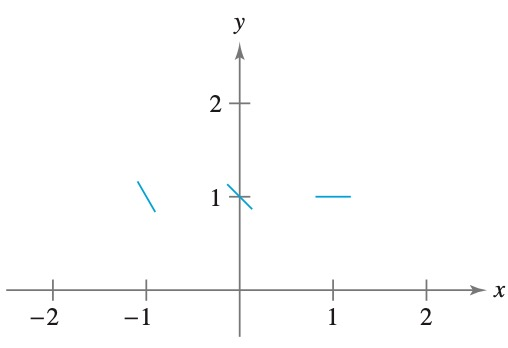
\includegraphics[width=0.45\linewidth]{Example_56.jpg} 
\end{minipage}
\end{tcolorbox}

\begin{tcolorbox}[colback=examplebg, colframe=red!75!black, title=\textbf{EXAMPLE 3: Sketching a Solution Using a Slope Field
}, fonttitle=\bfseries, sharp corners]
Sketch a slope field for the differential equation:
\[
y' = 2x + y.
\]
Use the slope field to sketch the solution that passes through the point \((1, 1)\).


\tcblower
\textbf{Solution:} 
Create a table showing the slopes at several points. The table below provides a small sample of calculations. The slopes at many other points should be calculated to get a representative slope field.

\[
\begin{array}{|c|c|c|c|c|c|c|c|c|c|c|}
\hline
x & -2 & -2 & -1 & -1 & 0 & 0 & 1 & 1 & 2 & 2 \\ \hline
y & -1 & 1  & -1 & 1  & -1 & 1 & -1 & 1 & -1 & 1 \\ \hline
y' = 2x + y & -5 & -3 & -3 & -1 & -1 & 1 & 1  & 3 & 3  & 5 \\ \hline
\end{array}
\]

These slopes can then be used to draw small line segments at the corresponding points to construct the slope field. The solution curve passing through \((1, 1)\) can be sketched using this slope field.

\begin{minipage}{\linewidth}
    \centering
    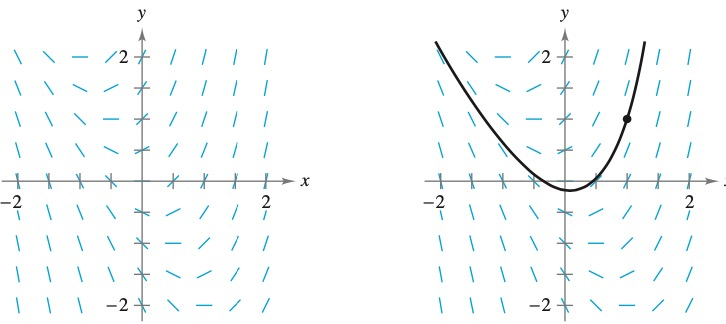
\includegraphics[width=0.60\linewidth]{Example_57.jpg} 
\end{minipage}
\end{tcolorbox}

\newpage

\subsection{Slope Field Analysis (Reasoning Using Slope Fields)}
 \textbf{Slope fields}, also known as direction fields, offer a visual approach to understanding the solutions of differential equations. 

\begin{Note}{Extracting Information from Slope Fields}{}
    A slope field provides a visual representation of a differential equation by showing the slope of the solution curve at various points. Each segment in the field represents the rate of change at a specific location, acting as a guide for how the solution behaves. By analyzing the direction and steepness of the slopes, we can infer patterns and trends in the solution to the differential equation.
\end{Note}

Consider the differential equation:
\[
y' = x + y.
\]
At specific points, the slopes are:
\[
\begin{array}{|c|c|c|c|}
\hline
(x, y) & (-1, 1) & (0, 0) & (1, -1) \\ \hline
y' = x + y & 0 & 0 & 0 \\ \hline
\end{array}
\]


These slopes can be used to sketch the slope field, revealing the overall behavior of the solution.

\begin{Note}{Using Slope Fields to Find Critical Points}{}
Critical points occur where the slope of the function is zero or undefined. In slope fields, these are shown by horizontal line segments (slope = 0) or vertical undefined slopes.
\end{Note}

\begin{tcolorbox}[colback=examplebg, colframe=red!75!black, title=\textbf{EXAMPLE 1: Find the Critical Point of the Differential Equation}, fonttitle=\bfseries, sharp corners]
For the differential equation:
\[
\frac{dy}{dx} = x - y,
\]
critical points occur where:
\[
x - y = 0 \quad \implies \quad y = x.
\]
The slope field will show horizontal lines along \(y = x\), indicating potential critical points.

\end{tcolorbox}


\begin{Note}{Solutions as Families of Functions}{}
When solving differential equations, the constant of integration \(+C\) introduces a family of solutions. This constant represents an arbitrary value added during integration, allowing for infinitely many solutions that differ by this constant.

\begin{minipage}{\linewidth}
    \centering
    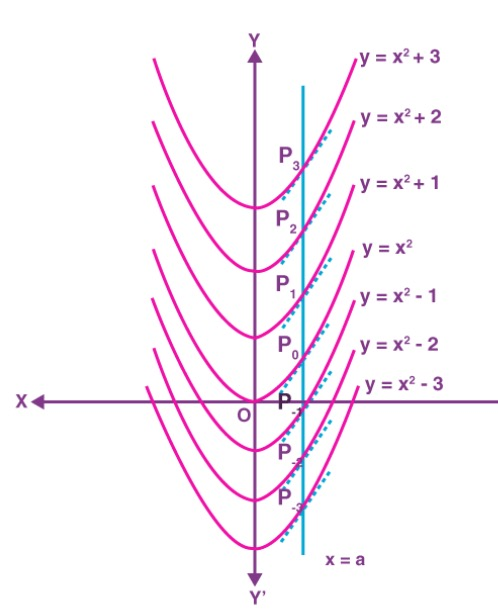
\includegraphics[width=0.40\linewidth]{Example_58.jpg} 
\end{minipage}

\end{Note}


\begin{tcolorbox}[colback=examplebg, colframe=red!75!black, title=\textbf{EXAMPLE 2: Find the Integral of the Function}, fonttitle=\bfseries, sharp corners]

Solve the differential equation:
\[
\frac{dy}{dx} = 2x.
\]

\tcblower
\textbf{Solution:} 
Integrating both sides:
\[
y = \int 2x \, dx = x^2 + C,
\]
where \(C\) is the constant of integration. This represents a family of parabolic solutions, each differing by the value of \(C\).
\end{tcolorbox}


\begin{tcolorbox}[colback=examplebg, colframe=red!75!black, title=\textbf{EXAMPLE 3: Slope Field and Solution}, fonttitle=\bfseries, sharp corners]
The slope field for a certain differential equation is shown. Which of the following could be a solution to the differential equation with the initial condition \(y(0) = 1\)?

\begin{enumerate}[(A)]
    \item \(y = \frac{x}{y} + 1\)
    \item \(y = -\frac{x}{y} + 1\)
    \item \(x^2 + (y + 1)^2 = 4\)
    \item \(x^2 + y^2 = 1\)
\end{enumerate}

\begin{minipage}{\linewidth}
    \centering
    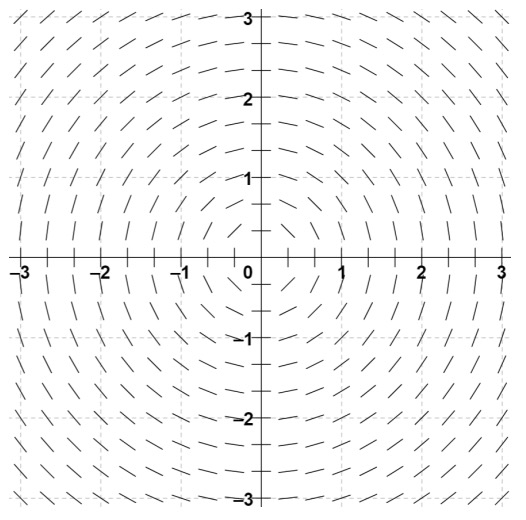
\includegraphics[width=0.40\linewidth]{Example_59.jpg} 
\end{minipage}


\tcblower
\textbf{Solution:} 
From the slope field, the curves appear circular and symmetric about the origin. Among the given options, the equation:
\[
x^2 + y^2 = 1
\]
represents a circle of radius 1, which matches the behavior of the slope field. Additionally, it satisfies the initial condition \(y(0) = 1\), as substituting \(x = 0\) yields \(y^2 = 1\), giving \(y = 1\) (the positive root).

Thus, the correct answer is:
\[
\boxed{D}
\]
\end{tcolorbox}



\begin{tcolorbox}[colback=examplebg, colframe=red!75!black, title=\textbf{EXAMPLE 4: Slope Field Analysis}, fonttitle=\bfseries, sharp corners]

The slope field for a certain differential equation is shown above. Which of the following statements about a solution \(y = f(x)\) to the differential equation must be false?

\begin{enumerate}[(A)]
    \item The graph of the particular solution that satisfies \(f(2) = -2\) has a relative minimum at \(x = 2\).
    \item \textbf{The graph of the particular solution that satisfies \(f(-1) = -1\) is concave up on the interval \(-2 < x < 1\).}
    \item The graph of the particular solution that satisfies \(f(1) = -2\) is linear.
    \item The graph of the particular solution that satisfies \(f(-1) = 2\) is concave up on the interval \(-3 < x < 3\).
\end{enumerate}

\begin{minipage}{\linewidth}
    \centering
    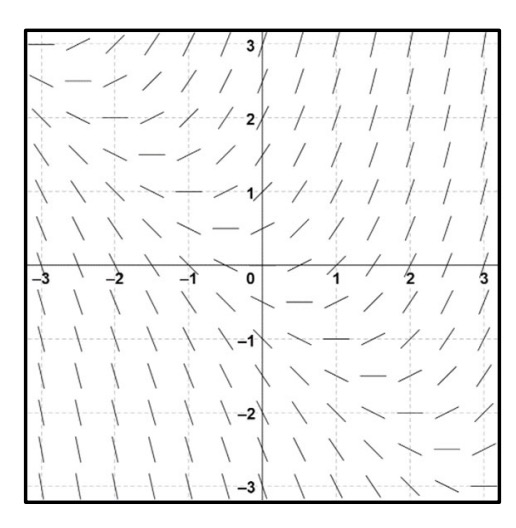
\includegraphics[width=0.40\linewidth]{Example_60.jpg} 
\end{minipage}

\tcblower
\textbf{Solution:} 
Looking at the slope field:
\begin{itemize}
    \item Statement (A) could be true because the slope around \(x = 2\) supports the behavior of a relative minimum.
    \item Statement (B) must be false because the slope field does not consistently indicate concavity upwards (\(y'' > 0\)) in the interval \(-2 < x < 1\).
    \item Statement (C) could be true since the solution might appear linear in this region based on the slope field.
    \item Statement (D) could also be true as the slope field suggests upward concavity on the interval \(-3 < x < 3\).
\end{itemize}

Thus, the correct answer is:
\[
\boxed{\text{B}}
\]
\end{tcolorbox}



\subsection{Approximating Solutions Using Euler’s Method}
\begin{Note}{BC ONLY}{}
    This is an AP Calculus BC topic only
\end{Note}

\begin{Definition}{Euler’s Method}{}
    \textbf{Euler's Method} is a numerical approach to approximating the particular solution of the differential equation:
\[
y' = F(x, y)
\]
that passes through the point \((x_0, y_0)\).

We can approximate a function as a set of line segments using Euler’s method


\begin{minipage}{\linewidth}
    \centering
    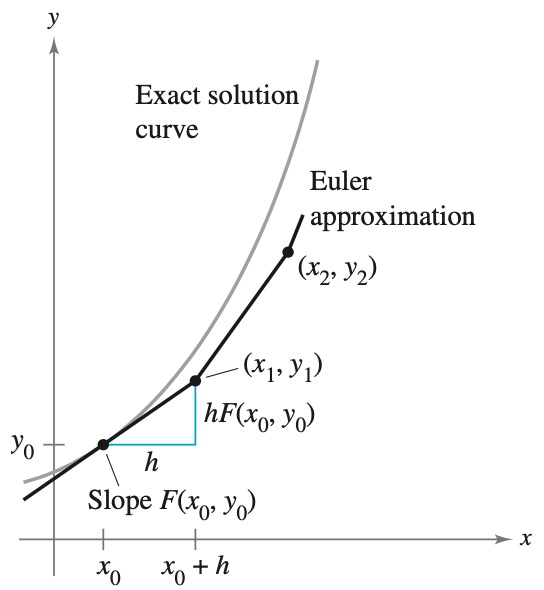
\includegraphics[width=0.40\linewidth]{Example_61.jpg} 
\end{minipage}
\end{Definition}


\begin{Note}{Formula of Euler’s Method }{}
    Given the initial conditions \((x_0, y_0)\), the solution is approximated iteratively using the formula:
\[
y_{n+1} = y_n + h \cdot F(x_n, y_n),
\]
where:
\begin{itemize}
    \item \(h\) is the step size,
    \item \(x_{n+1} = x_n + h\),
    \item \(F(x, y)\) is the derivative provided by the differential equation.
\end{itemize}

\end{Note}


\begin{tcolorbox}[colback=examplebg, colframe=red!75!black, title=\textbf{EXAMPLE 1: Approximating a Solution Using Euler's Method}, fonttitle=\bfseries, sharp corners]

Use Euler's Method to approximate the particular solution of the differential equation:
\[
y' = x - y,
\]
passing through the point \((0, 1)\). Use a step size of \(h = 0.1\).

\tcblower
\textbf{Solution:} 
Given:
\[
x_0 = 0, \quad y_0 = 1, \quad h = 0.1, \quad F(x, y) = x - y,
\]
we calculate the first three approximations as follows:

1. For \(n = 1\):
\[
y_1 = y_0 + h \cdot F(x_0, y_0) = 1 + 0.1 \cdot (0 - 1) = 0.9.
\]

2. For \(n = 2\):
\[
y_2 = y_1 + h \cdot F(x_1, y_1) = 0.9 + 0.1 \cdot (0.1 - 0.9) = 0.82.
\]

3. For \(n = 3\):
\[
y_3 = y_2 + h \cdot F(x_2, y_2) = 0.82 + 0.1 \cdot (0.2 - 0.82) = 0.758.
\]

\textbf{Table of Approximations}
The first ten approximations are shown in the table below:

\[
\begin{array}{|c|c|c|}
\hline
n & x_n & y_n \\
\hline
0 & 0.0 & 1.000 \\
1 & 0.1 & 0.900 \\
2 & 0.2 & 0.820 \\
3 & 0.3 & 0.758 \\
4 & 0.4 & 0.712 \\
5 & 0.5 & 0.681 \\
6 & 0.6 & 0.663 \\
7 & 0.7 & 0.657 \\
8 & 0.8 & 0.661 \\
9 & 0.9 & 0.675 \\
10 & 1.0 & 0.697 \\
\hline
\end{array}
\]

\textbf{Graph of the Approximate Solution}
The approximate solution can be plotted alongside the exact solution. The exact solution is:
\[
y = x - 1 + 2e^{-x}.
\]


\end{tcolorbox}


\newpage

\subsection{Finding General Solutions Using Separation of Variables}
\begin{Definition}{separable equation}{}
    A \textbf{separable equation} is a first-order differential equation in which the expression for \(\frac{dy}{dx}\) can be factored as a function of \(x\) times a function of \(y\). In other words, it can be written in the form:
\[
\frac{dy}{dx} = g(x)f(y).
\]
\end{Definition}


The name \textbf{separable} comes from the fact that the expression on the right side can be ``separated'' into a function of $x$ and a function of $y$. Equivalently, if $f(y) \neq 0$, we could write
\[
\frac{dy}{dx} = \frac{g(x)}{h(y)},
\]
where \(h(y) \neq 0\). To solve, the equation is rewritten in the differential form:
\[
h(y) \, dy = g(x) \, dx.
\]
This allows the variables \(x\) and \(y\) to be separated on opposite sides. Both sides are then integrated:
\[
\int h(y) \, dy = \int g(x) \, dx.
\]
The solution may define \(y\) implicitly or explicitly in terms of \(x\).

\begin{tcolorbox}[colback=examplebg, colframe=red!75!black, title=\textbf{EXAMPLE 1: }, fonttitle=\bfseries, sharp corners]

\[
\begin{array}{|c|c|}
\hline
\textbf{Original Differential Equation} & \textbf{Rewritten with Variables Separated} \\
\hline
x^2 + 3y \frac{dy}{dx} = 0 & 3y \, dy = -x^2 \, dx \\
\hline
(\sin x)y' = \cos x & dy = \cot x \, dx \\
\hline
\frac{x y'}{e^y + 1} = 2 & \frac{1}{e^y + 1} \, dy = \frac{2}{x} \, dx \\
\hline
\end{array}
\]


\end{tcolorbox}


\newpage
\begin{tcolorbox}[colback=examplebg, colframe=red!75!black, title=\textbf{EXAMPLE 2: Solved Differential Equations}, fonttitle=\bfseries, sharp corners]

\[
\frac{dy}{dx} = \frac{3x^2}{y}
\]

\tcblower
\textbf{Solution:} 
\[
y \, dy = 3x^2 \, dx
\]
\[
\frac{1}{2}y^2 = x^3 + C
\]
\[
y^2 = 2x^3 + C
\]
\[
y = \pm \sqrt{2x^3 + C}
\]
\end{tcolorbox}


\begin{tcolorbox}[colback=examplebg, colframe=red!75!black, title=\textbf{EXAMPLE 3: Solved Differential Equations}, fonttitle=\bfseries, sharp corners]
\[
\frac{dy}{dx} = 8x^2y
\]



\tcblower
\textbf{Solution:} 
\[
\frac{1}{y} \, dy = 8x^2 \, dx
\]
\[
\ln|y| = \frac{8}{3}x^3 + C
\]
\[
y = e^{\frac{8}{3}x^3 + C}
\]
\[
y = Ce^{\frac{8}{3}x^3}
\]
\end{tcolorbox}



\begin{tcolorbox}[colback=examplebg, colframe=red!75!black, title=\textbf{EXAMPLE 4: Solved Differential Equations}, fonttitle=\bfseries, sharp corners]

\[
\frac{dy}{dx} = (y+5)(x+2)
\]

\tcblower
\textbf{Solution:} 
\[
\frac{1}{y+5} \, dy = (x+2) \, dx
\]
\[
\ln|y+5| = \frac{x^2}{2} + 2x + C
\]
\[
y+5 = e^{\frac{x^2}{2} + 2x + C}
\]
\[
y = Ce^{\frac{x^2}{2} + 2x} - 5
\]

\end{tcolorbox}

\newpage

\subsection{Finding Particular Solutions Using Initial Conditions and Separation of Variables}

\begin{Note}{Difference Between General and Particular Solutions}{}
    \textbf{General Solution}

\vspace{1mm}
    
A \textbf{general solution} to a differential equation is a family of functions that satisfies the equation. There are infinitely many functions that could do so.


\vspace{5mm}


\textbf{Particular Solution}

\vspace{1mm}

A \textbf{particular solution} is a unique solution that passes through a specific point. It can be calculated when initial conditions are provided.
\end{Note}


When asking to write an expression, you must include the initial condition. Here is a general form that you can use:

\[
F(x) = y_0 + \int_a^x f(t) \, dt
\]

This is a particular solution to the differential equation 
\[
\frac{dy}{dx} = f(x),
\]
where $F(a) = y_0$ (the initial condition).

\begin{Note}{Solving a Separation of Variables Problem with Initial Conditions}{}
    \begin{enumerate}
    \item \textbf{Separate} the two variables that you will be using. For example, gather all the $x$'s on one side and $y$'s on the other side.
    \item \textbf{Integrate} both sides of the equation with respect to their variables. Make sure not to forget to add the $+C$!
    \item \textbf{Solve} for $y$ to get the general equation.
    \item \textbf{Plug in} your initial conditions (which are given!) for $x$ and $y$ and solve for $C$.
    \item Finally, \textbf{plug back in} your $C$ that you calculated and there’s your particular solution!
\end{enumerate}
\end{Note}





\begin{tcolorbox}[colback=examplebg, colframe=red!75!black, title=\textbf{EXAMPLE 1: Finding a Particular Solution}, fonttitle=\bfseries, sharp corners]
Given the differential equation:
\[
xy \, dx + e^{-x}(y^2 - 1) \, dy = 0,
\]
and the initial condition $y(0) = 1$.


\tcblower
\textbf{Solution:} 
Rearrange and separate variables:
\[
e^{-x}(y^2 - 1) \, dy = -xy \, dx.
\]
Integrate both sides:
\[
\int \frac{y}{y^2 - 1} \, dy = -\int x e^x \, dx.
\]
The solution to the integrals is:
\[
\frac{y^2}{2} - \ln|y| = -\frac{e^x}{2} + C.
\]
Substituting $y(0) = 1$, solve for $C$, and simplify to find the particular solution.
\end{tcolorbox}


\begin{tcolorbox}[colback=examplebg, colframe=red!75!black, title=\textbf{EXAMPLE 2: Population Model}, fonttitle=\bfseries, sharp corners]
The rate of change of a population $N(t)$ is proportional to $650 - N$, where $t$ is time in years. Initially, $N(0) = 300$, and $N(2) = 500$. Find $N(3)$.


\tcblower
\textbf{Solution:} 
Write the differential equation:
\[
\frac{dN}{dt} = k(650 - N).
\]
Separate variables:
\[
\frac{dN}{650 - N} = k \, dt.
\]
Integrate both sides:
\[
-\ln|650 - N| = kt + C.
\]
Solve for $N$:
\[
N = 650 - Ce^{-kt}.
\]
Use initial conditions to find $C$ and $k$, then calculate $N(3)$:
\[
N(3) \approx 552.
\]
\end{tcolorbox}


\newpage

\subsection{Exponential Models with Differential Equations}

\subsubsection{Growth and Decay Models}
In many applications, the rate of change of a variable $y$ is proportional to the value of $y$. When $y$ is a function of time $t$, the proportion can be written as:

\[
\frac{dy}{dt} = ky
\]

\noindent where $k$ is the proportionality constant.


\begin{mytheorem}{Exponential Growth and Decay Model}{}


If $y$ is a differentiable function of $t$ such that $y > 0$ and $\frac{dy}{dt} = ky$ for some constant $k$, then:

\[
y = Ce^{kt}
\]

\noindent where $C$ is the \textit{initial value} of $y$, and $k$ is the \textit{proportionality constant}. 

\textbf{Exponential growth} occurs when $k > 0$, and \textbf{exponential decay} occurs when $k < 0$.
\end{mytheorem}

\begin{tcolorbox}[colback=examplebg, colframe=red!75!black, title=\textbf{EXAMPLE 1: Using an Exponential Growth Model }, fonttitle=\bfseries, sharp corners]

The rate of change of $y$ is proportional to $y$. When $t = 0$, $y = 2$, and when $t = 2$, $y = 4$. What is the value of $y$ when $t = 3$?

\tcblower
\textbf{Solution:} 

Because $\frac{dy}{dt} = ky$, the solution can be expressed as:

\[
y = Ce^{kt}
\]

where $C$ and $k$ are constants. Using the given initial conditions, we solve for $C$ and $k$:

\[
2 = Ce^0 \quad \Rightarrow \quad C = 2
\]

Substitute $C$ into the equation. When $t = 2$, $y = 4$:

\[
4 = 2e^{2k} \quad \Rightarrow \quad e^{2k} = 2 \quad \Rightarrow \quad k = \frac{1}{2} \ln 2 \approx 0.3466
\]

Thus, the model becomes:

\[
y = 2e^{0.3466t}
\]

Finally, to find $y$ when $t = 3$:

\[
y = 2e^{0.3466(3)} \approx 2 \times 2.8285 \approx 5.657
\]

Therefore, $y \approx 5.657$ when $t = 3$.



\end{tcolorbox}


\begin{tcolorbox}[colback=examplebg, colframe=red!75!black, title=\textbf{EXAMPLE 2: 
Using an Exponential Growth Model}, fonttitle=\bfseries, sharp corners]
A radioactive substance has a rate of decay that can be modeled by the equation 
    \[
    \frac{dy}{dt} = ky,
    \]
    where $k$ is a constant and $t$ is measured in years. If the half-life of the radioactive substance is $300$ years, then what is the value of $k$?


\tcblower
\textbf{Solution:} 
    At $t = 300$, $y = \frac{1}{2}$, so:
    \[
    \frac{1}{2} = e^{k(300)}.
    \]
    Taking the natural logarithm of both sides:
    \[
    \ln\left(\frac{1}{2}\right) = 300k.
    \]
    Simplifying:
    \[
    k \approx -0.0023.
    \]
\end{tcolorbox}


\begin{tcolorbox}[colback=examplebg, colframe=red!75!black, title=\textbf{EXAMPLE 3: Using an Exponential Growth Model}, fonttitle=\bfseries, sharp corners]

A dose of $100$ milligrams of a drug is administered to a patient. The amount of the drug, in milligrams, in the person’s bloodstream at time $t$, in hours, is given by $A(t)$. The rate at which the drug leaves the bloodstream can be modeled by the differential equation
    \[
    \frac{dA}{dt} = -0.5A.
    \]
    Write an expression for $A(t)$.

\tcblower
\textbf{Solution:} 
    The general solution to the differential equation is:
    \[
    A(t) = Ce^{-0.5t}.
    \]
    Using the initial condition $A(0) = 100$:
    \[
    100 = Ce^{0}.
    \]
    Therefore, $C = 100$, and the solution is:
    \[
    A(t) = 100e^{-0.5t}.
    \]
\end{tcolorbox}


\begin{tcolorbox}[colback=examplebg, colframe=red!75!black, title=\textbf{EXAMPLE 4: Newton’s Law of Cooling}, fonttitle=\bfseries, sharp corners]

Let $y$ represent the temperature (in °F) of an object in a room whose temperature is kept at a constant $60^\circ$. The object cools from $100^\circ$ to $90^\circ$ in $10$ minutes. How much longer will it take for the temperature of the object to decrease to $80^\circ$?

\tcblower
\textbf{Solution:} 

From Newton's Law of Cooling, you know that the rate of change in $y$ is proportional to the difference between $y$ and $60$. This can be written as:
\[
\frac{dy}{dt} = k(y - 60), \quad 80 \leq y \leq 100.
\]
To solve this differential equation, use separation of variables, as shown:
\[
\frac{1}{y - 60} \, dy = k \, dt.
\]
\[
\int \frac{1}{y - 60} \, dy = \int k \, dt.
\]
\[
\ln|y - 60| = kt + C_1.
\]
Because $y > 60$, $|y - 60| = y - 60$, and you can omit the absolute value signs. Using exponential notation, you have:
\[
y - 60 = e^{kt + C_1},
\]
\[
y = 60 + Ce^{kt}.
\]
Now, use the initial condition $y = 100$ when $t = 0$ to find $C$:
\[
100 = 60 + C e^{k(0)} = 60 + C \quad \Rightarrow \quad C = 40.
\]
Next, use $y = 90$ when $t = 10$ to find $k$:
\[
90 = 60 + 40e^{k(10)} \quad \Rightarrow \quad 30 = 40 e^{10k} \quad \Rightarrow \quad e^{10k} = \frac{3}{4}.
\]
Taking the natural logarithm of both sides:
\[
10k = \ln \left(\frac{3}{4}\right) \quad \Rightarrow \quad k = \frac{1}{10} \ln \left(\frac{3}{4}\right) \approx -0.02877.
\]
Thus, the model is:
\[
y = 60 + 40 e^{-0.02877t}.
\]
\end{tcolorbox}


\subsection{Logistic Models with Differential Equations}

\begin{Definition}{Logistic Differential Equation}{}
The logistic growth model is a differential equation that describes population growth. It states that:

\begin{itemize}
    \item The growth rate of a population is proportional to both:
    \begin{enumerate}
        \item The current population size, and
        \item The difference between the population size and the carrying capacity.
    \end{enumerate}
    \item The carrying capacity is the maximum population size that the environment can support.
\end{itemize}

\begin{minipage}{\linewidth}
    \centering
    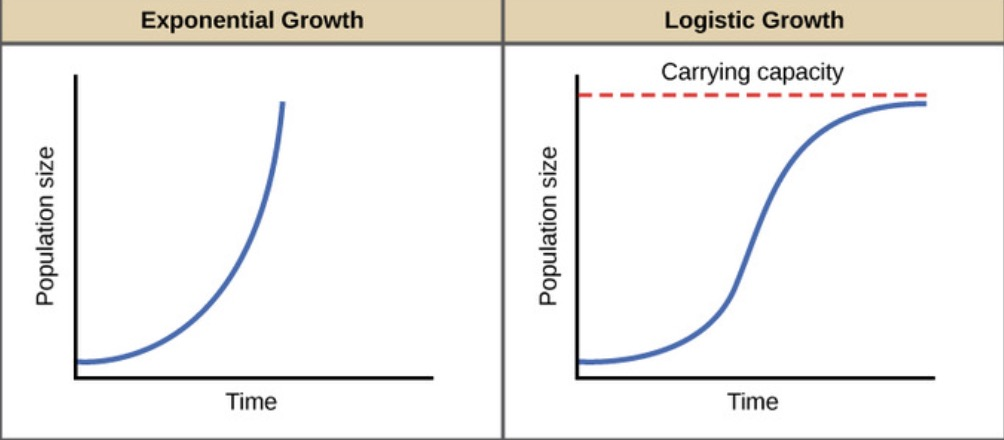
\includegraphics[width=0.65\linewidth]{Example_62.jpg} 
\end{minipage}
\end{Definition}


\begin{Note}{Logistic Differential Equation Formula}{}
    The logistic differential equation is given by:
\[
\frac{dy}{dt} = ky \left(1 - \frac{y}{L}\right)
\]

\begin{itemize}
    \item $k$ and $L$ are positive constants.
    \item $L$ is the \textbf{carrying capacity}, or the maximum population the environment can sustain.
    \item If $0 < y < L$, the population grows because $\frac{dy}{dt} > 0$.
    \item If $y > L$, the population decreases because $\frac{dy}{dt} < 0$.
\end{itemize}

The population stabilizes at $y = L$, forming a logistic curve.
\end{Note}




\begin{tcolorbox}[colback=examplebg, colframe=red!75!black, title=\textbf{EXAMPLE 1: Logistics Differential Equation}, fonttitle=\bfseries, sharp corners]
The function $P$ satisfies the logistic differential equation
\[
\frac{dP}{dt} = \frac{P}{20} \left(1 - \frac{P}{1700}\right),
\]
where $P(0) = 210$. Determine which of the following statements is \textbf{false}:

\begin{enumerate}
    \item $\lim_{t \to \infty} P(t) = 1700$ \hfill \checkmark
    \item $\frac{dP}{dt}$ has a maximum value when $P = 210$ \hfill \textbf{False}
    \item $\frac{d^2P}{dt^2} = 0$ when $P = 850$ \hfill \checkmark
    \item When $P > 850$, $\frac{dP}{dt} > 0$ and $\frac{d^2P}{dt^2} < 0$ \hfill \checkmark
\end{enumerate}


\tcblower
\textbf{Solution:} 
The maximum value of $\frac{dP}{dt}$ occurs at $P = \frac{L}{2}$, where $L = 1700$. Hence, the maximum occurs at $P = 850$ and not $P = 210$.
\end{tcolorbox}




\begin{tcolorbox}[colback=examplebg, colframe=red!75!black, title=\textbf{EXAMPLE 2: Logistics Differential Equation}, fonttitle=\bfseries, sharp corners]

The rate of change of the number of people entering an arena is modeled by a logistic differential equation. The capacity of the arena is $5000$ people. At a certain time, the number of people in the arena is $1000$, and the rate of increase is $500$ people per minute. Which of the following differential equations could describe this situation?

\[
\begin{aligned}
    \text{(A)} & \quad \frac{dP}{dt} = \frac{1}{800} (5000 - P) \\
    \text{(B)} & \quad \frac{dP}{dt} = \frac{1}{500} P (5000 - P) \\
    \text{(C)} & \quad \frac{dP}{dt} = \frac{1}{8000} P (5000 - P) \\
    \text{(D)} & \quad \frac{dP}{dt} = \frac{1}{5000} P (500 - P)
\end{aligned}
\]




\tcblower
\textbf{Solution:} 
\begin{align*}
    500 &= k(1000)(5000 - 1000), \\
    500 &= k(1000)(4000), \\
    k &= \frac{5}{8}.
\end{align*}

Thus, the differential equation is:
\[
\frac{dP}{dt} = \frac{1}{8000}P(5000 - P).
\]

\textbf{Answer:} \textbf{C.}
\end{tcolorbox}


\end{document}
